\documentclass[12pt, oneside, a4paper]{article}

% for math symbols
\usepackage{amsmath}
\usepackage{amssymb}
% for inserting images
\usepackage{graphicx}
% for algorithm pseudocode
\usepackage[noend]{algpseudocode}
\usepackage[nothing]{algorithm}
\algrenewcommand{\algorithmicrequire}{\textbf{Input:}}
\algrenewcommand{\algorithmicensure}{\textbf{Output:}}
\algnewcommand\And{\textbf{and} }
% for tables
\usepackage{tabularx}
% for implementation of the array and tabular environments
\usepackage{array}
% Control float placement. Defines a \FloatBarrier command
\usepackage{placeins}
% for derivative commands
\usepackage{physics}
% for multi level lists
\usepackage{outlines} 
% for links in text
\usepackage[colorlinks=true,linkcolor=blue,urlcolor=black,bookmarksopen=true]{hyperref}
% for contents after pdf is formed
\usepackage{bookmark}
% for caption
\usepackage[outercaption]{sidecap}
% for code
\usepackage{listings}
% for pictures
\usepackage{tikz}
\usepackage{indentfirst}


\def\nudge{.5}
\tikzset{axis/.style={ultra thick, black, -latex, shorten <=-\nudge cm, shorten >=-2*\nudge cm}}
\tikzset{line/.style={thick,green}}

\hypersetup{%
  colorlinks=true,
  linkcolor=blue,
  linkbordercolor={0 0 1}
}


\newcommand{\vect}[1]{\ensuremath{\mathbf{#1}}}
\newcommand{\vt}[1]{\ensuremath{\mathbf{#1}}}
\newcommand{\uline}[1]{\underline{#1}}
\newcommand{\tb}[1]{\textbf{#1}}
\newcommand{\ilcode}{\texttt}
\newcommand{\p}{\partial}
\newcommand{\vphi}{\varphi}
\newcommand{\ilc}{\texttt}

\DeclareUnicodeCharacter{2212}{\textendash}

\graphicspath{ {./images/} }


\begin{document} 
    \title{\textbf{ECSE 484 - Assignment 10}}
    \author{Oleksii Fedorenko and Cameroon Byrne}
    \maketitle
    
    Have you ever listened to a song and wondered what genre it is? Or have your ever though about what genre of songs you like to listen to? We ary trying to create a neural network that would answer both of those questions. We are gathering data from the Spotify api about the song characteristics and then use that as training data to train a network to recognize the genre of songs that you like. The song features that we can gather from Spotify are: danceability, energy, key, loudness, mode, speechiness, acousticness, instrumentalness, liveness, valence, and tempo. All of these values are floats and, combined together, are quite predictive of the song genre. We have already started designing a network that would be able to do the predictions for the genre.  
    
    \FloatBarrier 
    \begin{figure}[H]
        \caption{Data format} 
        \centerline{
        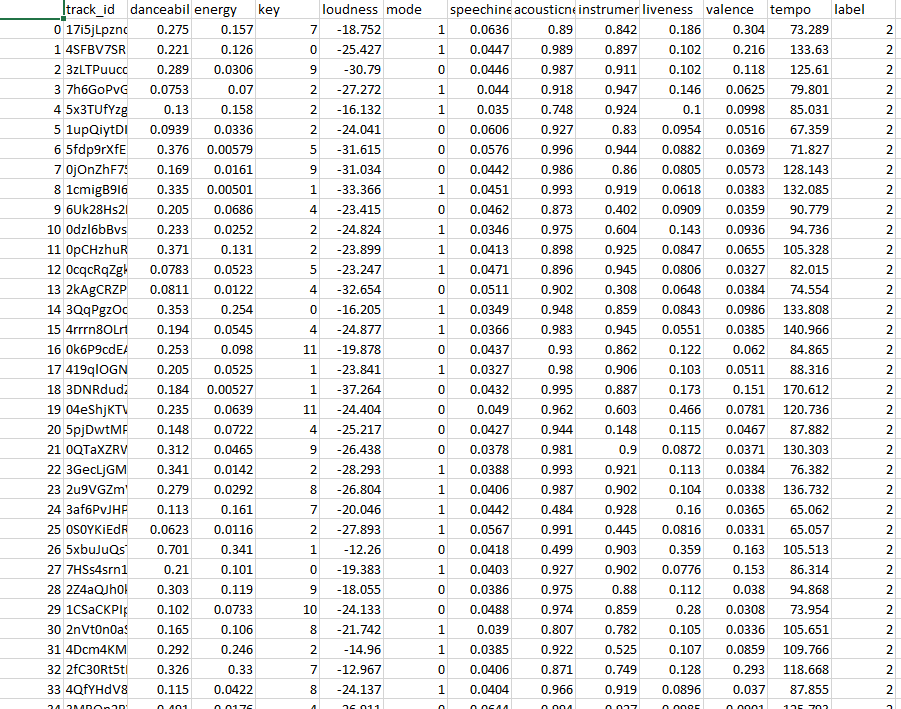
\includegraphics[width=\textwidth]{data.PNG}
        } 
    \end{figure}

    \FloatBarrier 
    \begin{figure}[H]
        \caption{Training set accuracy and loss} 
        \centerline{
        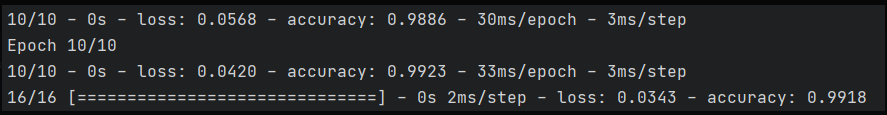
\includegraphics[width=\textwidth]{tarining_set_loss_acc.PNG}
        } 
    \end{figure}
    
    \FloatBarrier 
    \begin{figure}[H]
        \caption{Testing set accuracy and loss} 
        \centerline{
        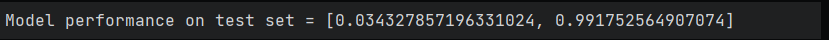
\includegraphics[width=\textwidth]{test_set.PNG}
        } 
    \end{figure}
    
    \FloatBarrier 
    \begin{figure}[H]
        \caption{The model that we used} 
        \centerline{
        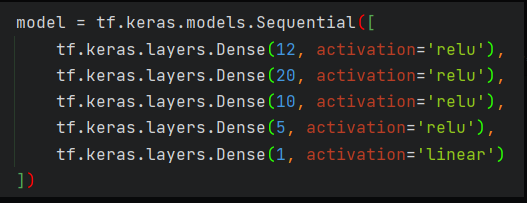
\includegraphics[width=\textwidth]{model.PNG}
        } 
    \end{figure}

    But we would not stop there. There are a couple of ideas we have in mind about how we can apply this data. For examply we can get a sample of songs from your favorite artist and album and determine their genre and mood. We would also try to make a neural network that would train on the data of the songs you like and a score you assign to train the network, rating the songs by how much you might like them and producing a ranking based on the predicted score for all of them. 
\end{document}